\chapter{Konzeption eines sicheren Capability-basierten Messaging-Systems (Vorbereitung der Masterarbeit)}
\label{chap:konzeption_messaging}

\section{Motivation: Sicherheitsdefizite bisheriger Delegationsmechanismen}

In einem strikten Capability-Betriebssystem wie D3OS dürfen Berechtigungen nicht über globale Tabellen verwaltet werden, stattdessen werden unfälschbare Zugriffstoken direkt im Dispatcher als Parameter übergeben. Die Delegierung (\textit{Sharing}) einer solchen Capability an einen anderen Prozess erfordert zwingend einen sicheren Transportkanal.

Im bisherigen Stand des Systems wurden für die Übertragung von Capabilities herkömmliche Pipes zweckentfremdet, was gravierende Sicherheits- und Architekturdefizite mit sich bringt:

\begin{itemize}
    \item \textbf{Mangelnde Zugriffsisolation:} Pipes besitzen keinen strikt prozessgebundenen Schutzraum; jeder Prozess, der einen Deskriptor auf die Pipe hält oder erlangt, kann Daten daraus lesen.
    \item \textbf{Abfanggefahr (Eavesdropping / Man-in-the-Middle):} Bei der Weitergabe von Capabilities über eine Pipe kann ein unautorisierter Dritter die übertragenen Rechte abfangen oder manipulieren, bevor der vorhergesehende Empfänger sie erhält.
    \item \textbf{Bruch des Capability-Prinzips:} Die Delegation erfolgt ungeschützt über einen Stream von Bytes, anstatt atomar und typisiert als eigenständiges Kernelobjekt übertragen zu werden.
\end{itemize}

Das übergeordnete Ziel der anstehenden Masterarbeit ist daher die vollständige Ablösung von Pipes durch ein synchrones, Capability-basiertes Messaging-System (IPC), über welches Capabilities direkt, atomar und isoliert zwischen Threads delegiert werden können.


\section{Analyse alternativer IPC-Ansätze}

Für mikrokerngestützte IPC-Systeme existieren in modernen Rust-Betriebssystemen unterschiedliche Ansätze, die im Vorfeld auf ihre Eignung für D3OS geprüft wurden:

\subsection{Hubris: Das Lease-Modell}

Das Betriebssystem Hubris nutzt sogenannte \textit{Leases}, bei denen der Sender dem Empfänger temporär Zugriff auf definierte Speicherbereiche gewährt.

\begin{itemize}
    \item \textbf{Hardware-Voraussetzung:} Hubris zielt primär auf eingebettete Systeme mit einer Memory Protection Unit (MPU) ab, die beliebige Speicherregionen mit variabler Größe und hardwarenahen Schutzmasken isolieren kann.
    \item \textbf{Inkompatibilität mit D3OS:} D3OS operiert auf Standard-x86\_64-Hardware mit einer Memory Management Unit (MMU) und vierstufiger Seitentabelle (PML4). Die MMU erzwingt eine feste Granularität von 4-KiB-Pages. Müsste ein Prozess einem Kommunikationspartner lediglich Zugriff auf eine 50-Byte-Struktur gewähren, erhielte dieser zwangsläufig Zugriff auf die gesamten verbleibenden 4046 Bytes der Page. Dies führt entweder zu erheblichem Overhead oder verletzt das Prinzip der minimalen Rechtevergabe.
\end{itemize}

\subsection{Xous: Page Swapping}

Das Mikrokern-Betriebssystem Xous realisiert größere IPC-Übertragungen durch \textit{Page Swapping}, indem eine physische Speicherseite aus dem virtuellen Adressraum des Senders aus- und in den des Empfängers eingehängt wird.

\begin{itemize}
    \item \textbf{Nachteile:} Auch hier erzwingt die MMU eine strikte 4-KiB-Ausrichtung (\textit{page-aligned}). Jeder User-Space-Datenpuffer müsste exakt an einer Page-Grenze beginnen. Dies erfordert hochkomplexe, dedizierte Allokatoren im User-Space und erzeugt bei kleinen Nachrichten ebenfalls massiven Overhead.
    \item \textbf{Architektur-Diskrepanz:} Xous nutzt zur Adressierung globale Prozess- bzw. Server-IDs, was fundamental dem Capability-Prinzip widersprechen würde.
\end{itemize}


\section{Das gewählte Paradigma: Der seL4-Ansatz}

Aufgrund der genannten Limitierungen lehnt sich das Entwurfskonzept für D3OS an das Messaging-Modell des verifizierten Mikrokerns seL4 an. Dieses Modell zeichnet sich durch drei Kernprinzipien aus:

\begin{itemize}
    \item \textbf{Synchroner Rendezvous-Mechanismus:} Es existiert kein unbeschränkter Zwischenpuffer im Kernel; der Datentransfer findet erst statt, wenn sowohl Sender als auch Empfänger bereit sind.
    \item \textbf{Strikte Trennung von Control Plane und Data Plane:}
    \begin{itemize}
        \item \textbf{Control Plane (Short IPC):} Kleine Steuernachrichten und Metadaten werden Zero-Copy direkt über die CPU-Register ausgetauscht.
        \item \textbf{Data Plane (Shared Memory):} Große Nutzdatenmengen werden über gemeinsam genutzten physikalischen Speicher transferiert, dessen Zugriff über Capabilities geregelt wird. Dies passt optimal zu D3OS, da Shared Memory bereits im Betriebssystem implementiert ist
    \end{itemize}
    \item \textbf{Pufferlose Endpoints:} Die Kommunikation wird über Endpoint-Kernelobjekte serialisiert, welche Warteschlangen für blockierte Threads verwalten.
\end{itemize}


\section{Kernkomponenten des Messaging-Systems}

Zur Vorbereitung auf die Implementierung wurden die notwendigen Kernel-Datenstrukturen entworfen. Abbildung~\ref{fig:endpoint_architecture} veranschaulicht die Komponenten zwischen den beteiligten Threads und dem Endpoint-Kernelobjekt.

\begin{figure}[htbp]
  \centering
  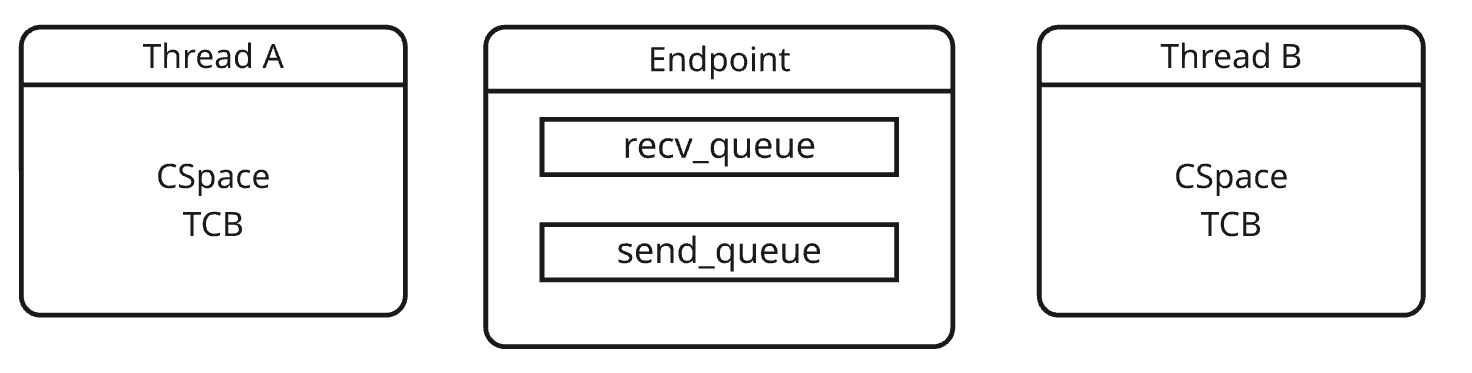
\includegraphics[width=0.95\textwidth]{img/endpoints.png}
  \caption{Architektur der Kernkomponenten und Endpoint-Interaktion.}
  \label{fig:endpoint_architecture}
\end{figure}

\subsection{Endpoints und Queues}

Ein Endpoint fungiert als reines Synchronisationstor und besitzt zwei interne Warteschlangen:

\begin{itemize}
    \item \texttt{recv\_queue}: Hält wartende Empfänger-Threads (Status: \texttt{BlockedOnReceive}).
    \item \texttt{send\_queue}: Hält wartende Sender-Threads (Status: \texttt{BlockedOnSend}).
\end{itemize}

\subsection{Thread Control Block (TCB) Erweiterungen}

Der TCB eines Threads wird um spezifische IPC-Felder ergänzt:

\begin{itemize}
    \item \texttt{ipc\_buffer}: Kein dynamisch allozierter Puffer im Kernel-Heap, sondern eine temporäre Speicherstelle für gesicherte CPU-Register (für den Short-IPC-Fall, falls ein Thread schlafen gelegt werden muss).
    \item \texttt{ipc\_cap}: Hält eine Kopie der zu delegierenden Capability aus dem senderseitigen CSpace.
    \item \texttt{badge}: Eine im CSpace des Senders hinterlegte ID, die der Kernel beim Transfer an den Empfänger durchreicht. Anhand dieses Badges kann ein Server eindeutig identifizieren, welcher Client die Nachricht gesendet hat.
\end{itemize}

\section{Der Rendezvous-Mechanismus im Detail}

Die Interaktion zwischen den Parteien gliedert sich in drei grundlegende Szenarien:

\paragraph{Szenario A: Empfänger wartet bereits (Server-Modus)}
\begin{enumerate}
    \item Thread B ruft \texttt{sys\_seL4\_Recv()} auf. Da keine Nachricht vorliegt, wird Thread B in die \texttt{recv\_queue} des Endpoints eingehängt und blockiert (\texttt{BlockedOnReceive}).
    \item Thread A setzt \texttt{sys\_seL4\_Send()} ab.
    \item Der Kernel stellt fest, dass in der \texttt{recv\_queue} bereits ein Empfänger wartet. Die \texttt{send\_queue} wird vollständig umgangen: Der Inhalt des \texttt{ipc\_buffer} bzw. der CPU-Register wird direkt von Thread A zu Thread B transferiert.
\end{enumerate}

\begin{figure}[htbp]
  \centering
  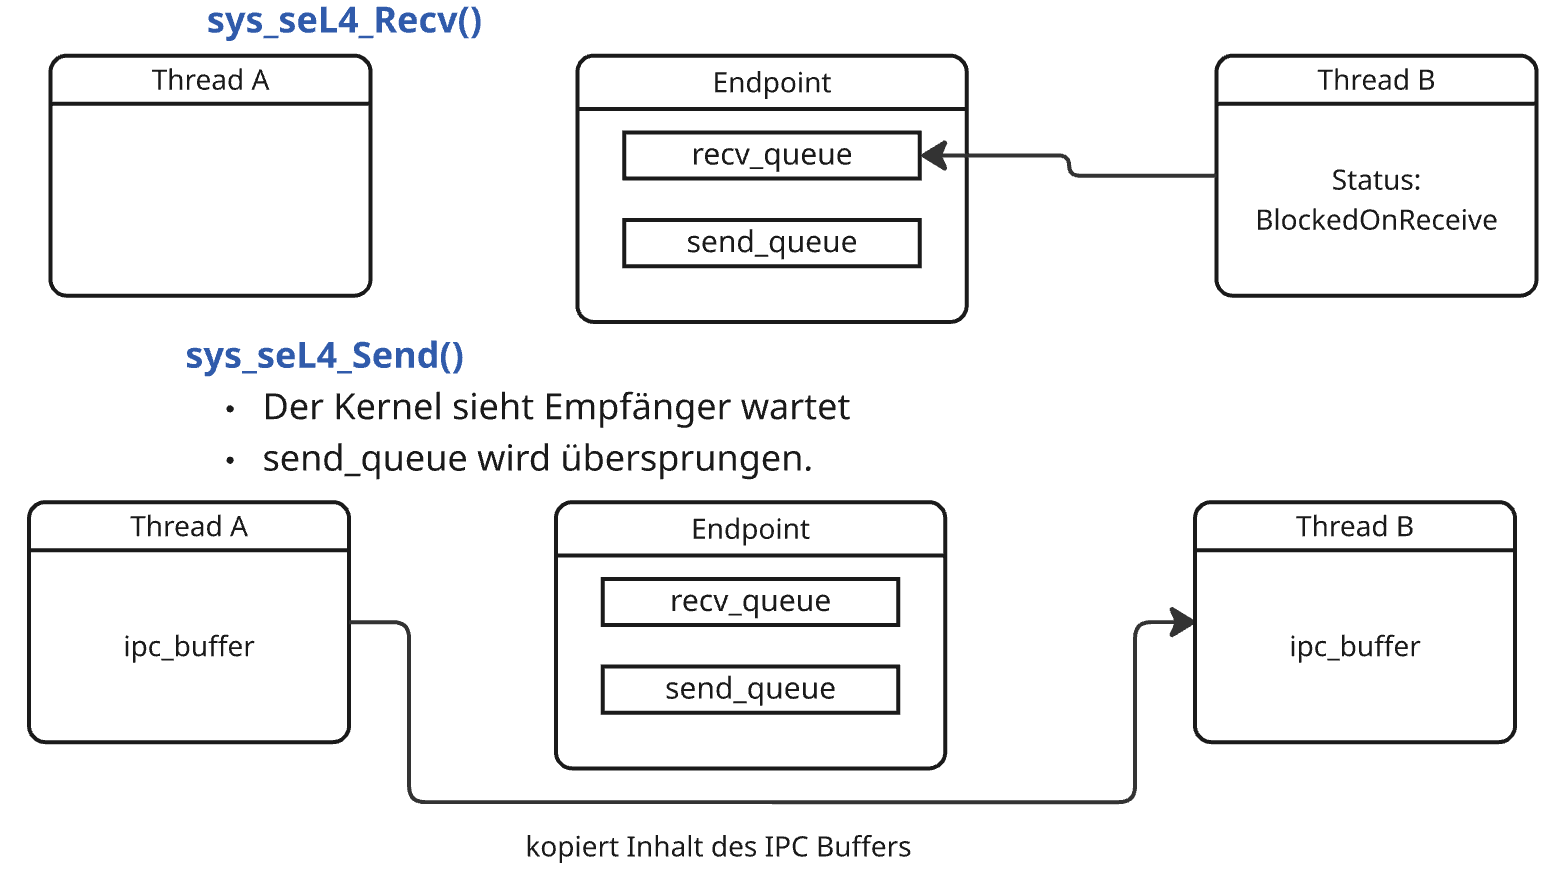
\includegraphics[width=0.85\textwidth]{img/receiver_waiting.png}
  \caption{Szenario A: Empfänger wartet bereits.}
  \label{fig:receiver_waiting}
\end{figure}

\paragraph{Szenario B: Sender trifft vor Empfänger ein (Client-Modus)}
\begin{enumerate}
    \item Thread A ruft \texttt{sys\_seL4\_Send()} auf. Der intendierte Empfänger horcht noch nicht am Endpoint.
    \item Thread A wird in den Zustand \texttt{BlockedOnSend} versetzt. Seine Registerinhalte werden im TCB (\texttt{ipc\_buffer}) gesichert, und Thread A wird in die \texttt{send\_queue} eingereiht.
    \item Sobald Thread B später \texttt{sys\_seL4\_Recv()} ausführt, erkennt der Kernel den wartenden Sender, weckt Thread A auf und überträgt die Daten aus dessen \texttt{ipc\_buffer} direkt in den Adressraum bzw. die Register von Thread B.
\end{enumerate}

\begin{figure}[htbp]
  \centering
  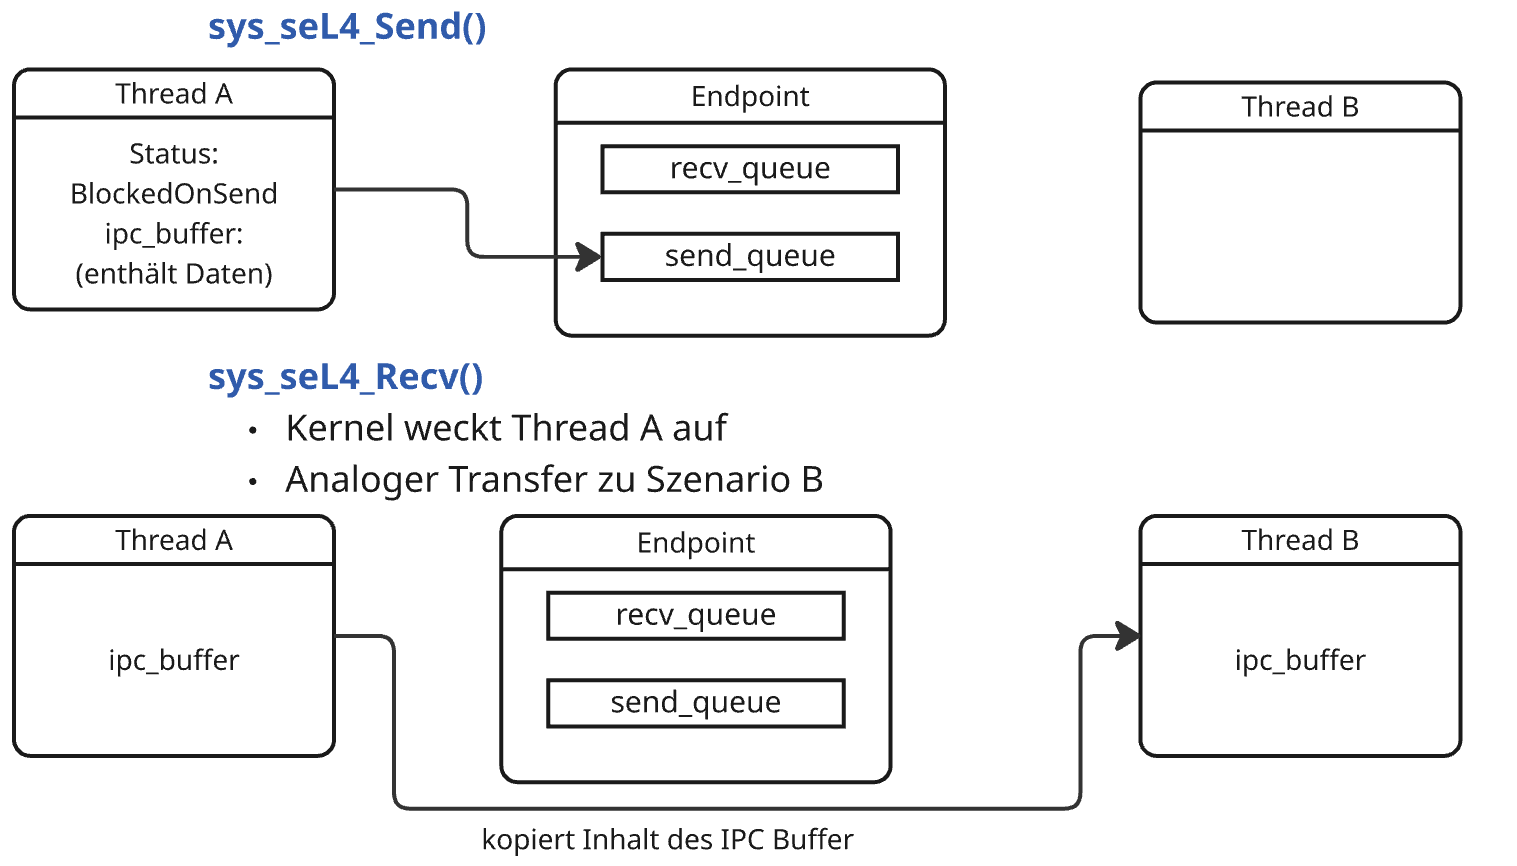
\includegraphics[width=0.85\textwidth]{img/sender_to_early.png}
  \caption{Szenario B: Sender trifft vor Empfänger ein.}
  \label{fig:sender_to_early}
\end{figure}

\paragraph{Szenario C: Delegation von Capabilities und Data Plane}
Sollen größere Datenmengen ausgetauscht werden, agiert das Messaging-System als Kontrollkanal:
\begin{enumerate}
    \item Thread A erzeugt eine Shared-Memory-Capability für einen definierten Speicherbereich und hinterlegt diese im TCB unter \texttt{ipc\_cap}.
    \item Beim Rendezvous prüft der Kernel die Gültigkeit der Capability und das gesetzte \texttt{SHARE}-Flag.
    \item Der Kernel klont die Capability autorisiert in den CSpace von Thread B.
    \item Nach Abschluss des Short-IPCs besitzen beide Threads eine valide Referenz auf denselben physikalischen RAM-Bereich. Große Payloads können nun ohne Beteiligung des Kernels direkt gelesen und geschrieben werden.
\end{enumerate}

\begin{figure}[htbp]
  \centering
  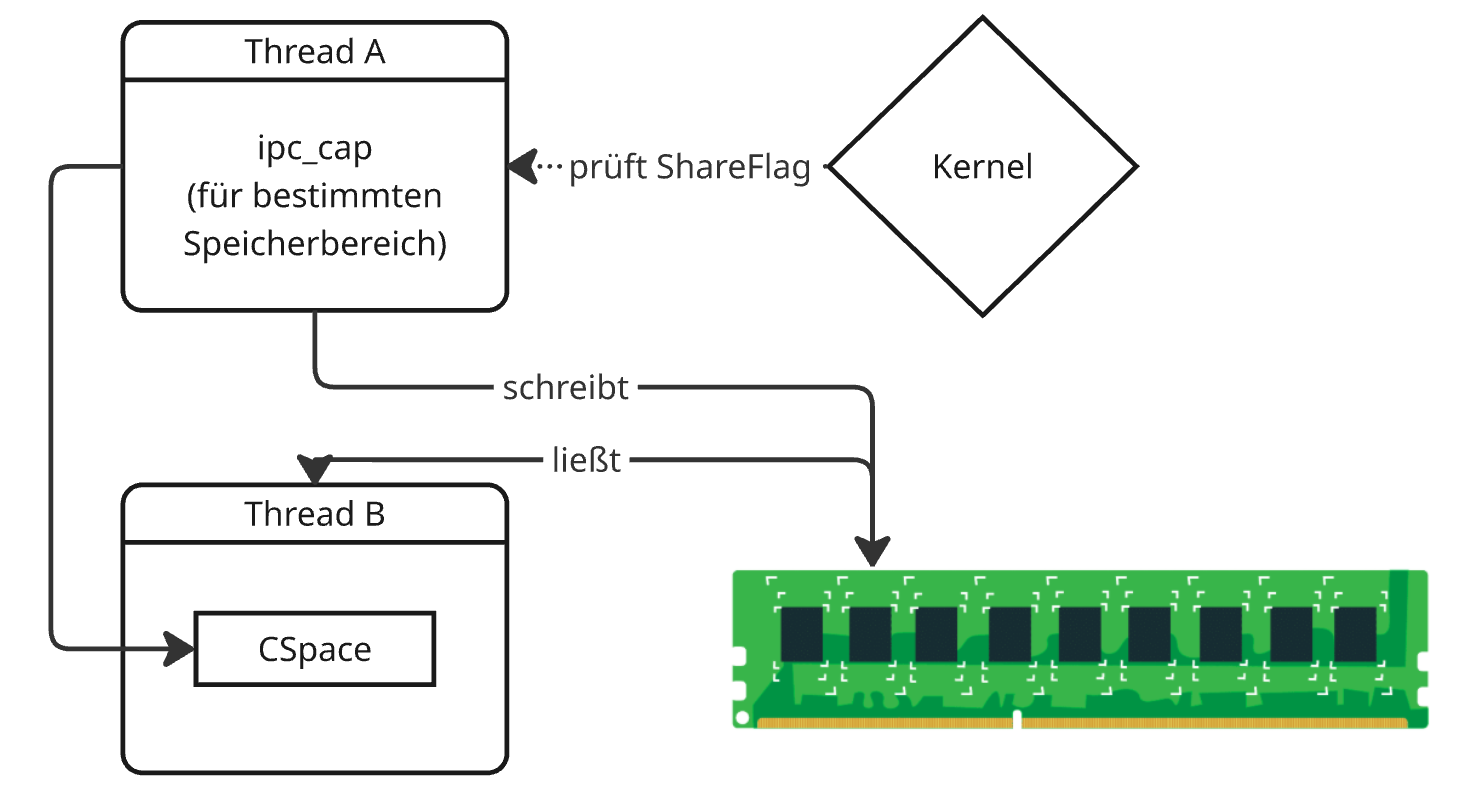
\includegraphics[width=0.85\textwidth]{img/shared_memory.png}
  \caption{Szenario C: Delegation von Capabilities und Data Plane.}
  \label{fig:shared_memory}
\end{figure}


\section{Optimierung: Regulärer Rust-Pfad vs. seL4 Assembler-Fastpath}

Für die Realisierung des Short-IPCs im Rahmen der Masterarbeit werden zwei Entwurfsvarianten evaluiert:

\usetikzlibrary{positioning}

\paragraph{Regulärer Rust-Pfad:}
\begin{center}
\begin{tikzpicture}[scale=0.92, transform shape,
  stepbox/.style={draw=hhuCorporateDarkBlue, rounded corners=2pt, fill=hhuCorporateGrey!20, font=\footnotesize, align=center, inner sep=4pt},
  flowarrow/.style={->, >=stealth, thick, color=hhuCorporateDarkBlue}
]
  \node[stepbox] (reg1) {Register};
  \node[stepbox, right=0.8cm of reg1] (stack) {Stack\\(RAM)};
  \node[stepbox, right=0.8cm of stack] (tcb) {TCB\\(RAM)};
  \node[stepbox, right=0.8cm of tcb] (reg2) {Register\\(Empfänger)};

  \draw[flowarrow] (reg1) -- node[above, font=\scriptsize] {Hardware-Trap} (stack);
  \draw[flowarrow] (stack) -- node[above, font=\scriptsize] {Rust-Logik} (tcb);
  \draw[flowarrow] (tcb) -- node[above, font=\scriptsize] {Kontextwechsel} (reg2);
\end{tikzpicture}
\end{center}

\paragraph{seL4 Assembler-Fastpath:}
\begin{center}
\begin{tikzpicture}[scale=0.92, transform shape,
  stepbox/.style={draw=hhuCorporateGreen!80!black, rounded corners=2pt, fill=hhuCorporateGreen!15, font=\footnotesize, align=center, inner sep=4pt},
  flowarrow/.style={->, >=stealth, thick, color=hhuCorporateGreen!80!black}
]
  \node[stepbox] (sender) {Register\\(Sender)};
  \node[stepbox, right=5.2cm of sender] (receiver) {Register\\(Empfänger)};

  \draw[flowarrow] (sender) -- node[above, font=\footnotesize] {Adressraum-Switch} node[below, font=\scriptsize\itshape] {(True Zero-Copy ohne RAM-Zugriff)} (receiver);
\end{tikzpicture}
\end{center}

\subsection*{Der reguläre Rust-Pfad}
Im regulären Rust-Pfad sichert die Hardware beim Wechsel in den Kernel die CPU-Register des Senders sofort auf dem Stack im RAM. Die Rust-Logik des Kernels liest diese Daten anschließend aus dem Arbeitsspeicher aus und kopiert sie intern in den Thread Control Block. Nach dem erfolgten Kontextwechsel holt die CPU die Daten wieder aus dem RAM und schreibt sie in die Register des Empfängers. Trotz der mehrfachen Speicherzugriffe ist dieser Ansatz deutlich einfacher zu implementieren und weitaus weniger fehleranfällig als komplexe Low-Level-Routinen. Er eignet sich daher ideal für einen ersten, stabilen Prototypen, um die Funktionalität des Messaging- und Delegationssystems zunächst isoliert und zuverlässig zu verifizieren.

\subsection*{Der seL4 Assembler-Fastpath}
Für synchrone Short-IPCs wird ein hochoptimierter Pfad in x86\_64-Assembly angestrebt:
\begin{itemize}
    \item Die Nachrichtendaten (z.\,B. Badges, Syscall-Argumente, Capability-Handles) verbleiben während des gesamten Wechsels physisch in den Allzweckregistern.
    \item Die Register behalten ihren Zustand, ohne umkopiert werden zu müssen.
    \item Der Empfänger erwacht mit den exakten Registerwerten des Senders und es findet kein einziger Lese- oder Schreibzyklus auf den RAM statt (\textit{True Zero-Copy}).
\end{itemize}


\section{Ausblick auf die Masterarbeit}

Die in dieser Projektarbeit durchgeführten Vorarbeiten schaffen das Fundament für die Masterarbeit. Zu diesen gehören die Optimierung der IPC Locks per \texttt{RwLock}, die Stabilisierung der Fehlerbehandlung im Syscall-Dispatcher, das Einpflegen des \texttt{SHARE}-Flags sowie die Vorbereitung der TCB- und CSpace-Strukturen.

Auf dieser Basis wird die konkrete Implementierung des seL4-orientierten Endpoint-Modells, der Assembler-Fastpath für Zero-Copy-Short-IPC sowie die vollständige Migration aller prozessübergreifenden Capability-Delegationen weg von unsicheren Pipes hin zum neuen Messaging-System erfolgen.
